%% LyX 2.2.1 created this file.  For more info, see http://www.lyx.org/.
%% Do not edit unless you really know what you are doing.
\documentclass{aghdpl}
\usepackage[T1]{fontenc}
\usepackage[utf8]{inputenc}
\setcounter{secnumdepth}{3}
\setcounter{tocdepth}{3}
\usepackage{verbatim}
\usepackage[unicode=true,pdfusetitle,
 bookmarks=true,bookmarksnumbered=true,bookmarksopen=true,bookmarksopenlevel=3,
 breaklinks=false,pdfborder={0 0 1},backref=false,colorlinks=false]
 {hyperref}
\usepackage{breakurl}

\makeatletter

%%%%%%%%%%%%%%%%%%%%%%%%%%%%%% LyX specific LaTeX commands.
%% Because html converters don't know tabularnewline
\providecommand{\tabularnewline}{\\}
\newcommand\tab[1][1cm]{\hspace*{#1}}
%%%%%%%%%%%%%%%%%%%%%%%%%%%%%% User specified LaTeX commands.
\usepackage{polski} 



\usepackage{mathtools}
\usepackage{amsfonts}
\usepackage{amsmath}
\usepackage{amsthm}

\usepackage[
style=numeric,
sorting=none,
language=autobib,
autolang=other,
urldate=iso8601,
backref=false,
isbn=true,
url=false,
maxbibnames=3,
backend=biber,
]{biblatex}
\usepackage{csquotes} 
\DeclareQuoteAlias{croatian}{polish} 


\addbibresource{bibliografia.bib}

\AtBeginDocument{

}

\author{SIMENS Healthkare}
\shortauthor{SIMENS}
\titlePL{DADM project documentation - draft}
\titleEN{}
\shorttitlePL{DADM project documentation}
\shorttitleEN{DADM project documentation}
\thesistype{}
\supervisor{PhD. Tomasz Pięciak}
\degreeprogramme{Biomedical engineering}
\date{2017}
\department{Department of  Automatics and Biomedical Engineering}
\faculty{AGH University of Science and Technology\protect\\[-2mm]
Faculty of Electrical Engineering, Automatics,\protect\\[-2mm] Computer Science and Biomedical Engineering}
\acknowledgements{}
\setlength{\cftsecnumwidth}{10mm}



\makeatother

\usepackage[english]{babel}
\begin{document}
\titlepages

\fancypagestyle{plain} {
	\fancyhf{}
	\renewcommand{\headrulewidth}{0pt}
	\renewcommand{\footrulewidth}{0pt}
}

\setcounter{tocdepth}{2}

\tableofcontents{}

\clearpage{}

\chapter{List of changes}

\begin{tabular}{|c|c|c|}
\hline 
Name & Date & Details\tabularnewline
\hline 
\hline 
Sylwia Mól & 19-Nov-2017 & Document created\tabularnewline
\hline 
 Sylwia Mól &  20-Nov-2017 & Structure changed\tabularnewline
\hline 
 Sylwia Mól &  21-Nov-2017 & Chapter "Authors" added, in-out table added\tabularnewline
\hline 
Malwina Molendowska  & 26-Nov-2017  & Description of 1st module added\tabularnewline
\hline 
Eliza Kowalczyk  & 27-Nov-2017  & Description of 9th module added\tabularnewline
\hline 
Karolina Gajewska & 27-Nov-2017  & Description of 10th module added\tabularnewline
\hline 
 &  & \tabularnewline
\hline 
\end{tabular}

\chapter{Assumptions}

about the app - the aim, what you can do here etc. 

\chapter{Structure}

dependences (tree), modules` descriptions
\\ 
\begin{tabular}{|c|c|c|c|}
\hline 
Module & Input  & Output & Before that module\tabularnewline
\hline 
\hline 
1& e.g. raw (subsampled) \textbf{k}-space signals & e.g. \textbf{x}-space fully reconstructed data  & --------\tabularnewline
\hline 
2& & &\tabularnewline
\hline 
3 &  & &\tabularnewline
\hline 
 4&  & &\tabularnewline
\hline
 5&  & &\tabularnewline
\hline 
 6&  & &\tabularnewline
\hline 
 8&  & &\tabularnewline
\hline 
9& 320x240 image & 640x480 image & denoised data \tabularnewline
\hline    
10 & 1)segmentated image 2)defined plane, image & 1)3D model (e.g. vtkPolyData) 2)cross-section image & 1)segmentation 2) denoised data\tabularnewline
\hline 
 11&  & &\tabularnewline
\hline  
\end{tabular}


\chapter{User guide}

\section{Requirements}
what user need to use this app - e.g. windows version etc

\section{Instruction}

instructions for user - GUI screens etc
\chapter{Detailed description}

\section{Module 1}

The aim of this module is to formulate mathematical algorithm, which enables proper
data reconstruction for images obtained with parallel MRI scans. The reconstruction is performed with use of Sensitivity Encoding (SENSE) algorithm in least squares (LS) solution context and Tikhonov regularization method. 

Generally, parallel MRI acquisitions are targeted to diminish time needed for data sampling. The usage of multiple coils enabled simultaneous acquisition of signals. A further step, which is acquiring partial data from \textbf{k}-space, leads to craved time savings, meanwhile maintaining full spatial resolution as well as contrast at the same time. However, the approach of omitting lines in acquisition step results in data aliasing, i.e. folded images that need further data processing.

To clearly mark out how data is processed in this module, we list following reconstruction steps: i) the application of 2D Fourier Transform transform (2D FFT) to \textbf{k}-space data (acquired raw signals) from multiple coils. The result is a set of \textbf{x}-space images with folded pixels, ii) the sensitivity maps estimation of coils profiles (the information is needed to properly unfold subsampled data) and iii) the proper unfolding data process with usage of SENSE reconstruction algorithm and its alterations.

The most crucial step in processing is estimation of sensitivity coil profiles as a successful image reconstruction with use of pMRI algorithms highly depends on accurate sensitivity coil assessment. As sensitivity information varies from scan to scan it is impossible to obtain absolute maps. To obtain reliable knowledge, reference
scans have to be conducted each time an examination is performed. These low-resolution information helps to estimate coil profiles with use of the many methods i.e. dividing each component coil image by a 'sum of squares' image.
 
It basic formulation, SENSE algorithm is applied to Cartesian MRI data undersampled uniformly by a factor $r$~(i.e. $r = 2$ means that every other line in \textbf{k}-space is skipped). After Fourier transformation, each pixel in \textbf{x}-space image received in \textit{l}-th coil can be seen as weighted sum of $r$ pixels from full FOV, each multiplied by corresponding localized values of maps. The distance between those 'aliased' points in the full FOV is always equal to the desired FOVy value divided by subsampling rate. Obviously, depending on subsampling rate the number of folded pixels changes. Basically, the signal in one pixel at a certain location $(x,y)$ received from $l$-th component coil image $D_{l}^{S}$ with chosen subsampling rate $r$ can be written as:
\begin{equation}
D_{l}^{S} (x,y) =  S_{l}(x,y_{1})D^{R}(x,y_{1}) + S_{l}(x,y_{2})D^{R}(x,y_{2}) + ... + S_{l}(x,y_{r})D^{R}(x,y_{r}),
\label{Eq:wzor1}
\end{equation}
where index $l$ counts from 1 to $L$ (number of coils) and index $i$ counts from 1 to $r$. Eq.(\ref{Eq:wzor1}) can be rewritten as:

\begin{equation}
D_{l}^{S} (x,y) = \sum_{i=1}^{r} S_{l}(x,y_{i})D^{R}(x,y_{i}) \quad     \text{for}  \quad  l = 1, ..., L.
\label{Eq:wzor2}
\end{equation}

Including all $L$ coils the above equation can be rewritten in a matrix form:

\begin{equation}
\textbf{D}^{S} (\textbf{x}) =  \textbf{S}(\textbf{x})\textbf{D}^{R} (\textbf{x}),
\label{Eq:wzor3}
\end{equation}

The vector $\textbf{D}^{S} (\textbf{x})$ denotes the aliased coil image values at a specific location \textbf{x} = $(x,y_{i})$ and has a length of $L$, $\textbf{S}(\textbf{x})$ is a $L$x$R$ matrix and represents the sensitivities values for each coil at the $r$~superimposed positions and $\textbf{D}^{R} (\textbf{x})$ lists the $r$ pixels from full FOV image to be reconstructed. The closed-form solution of the problem is as follows:
\begin{equation}
\widehat{\textbf{D}^{R}(\textbf{x})}= (\textbf{S}^{H}(\textbf{x})\textbf{S}(\textbf{x}))^{-1}\textbf{S}^{H}(\textbf{x})\textbf{D}^{S}(\textbf{x}),
\label{Eq:wzor4}
\end{equation}
where $\widehat{\textbf{D}^{R} (\textbf{x})} =  [\widehat{D^{R} (x,y_{1})}, ..., \widehat{D^{R} (x,y_{r})}]^{T}$ and $\textbf{S}^{H}(\textbf{x})$ is the conjugate transpose of the $\textbf{S}(\textbf{x})$ matrix. The final reconstruction image is defined as:
\begin{equation}
M(\textbf{x}) = \left |\widehat{\textbf{D}^{R}(\textbf{x})}  \right |.
\label{Eq:wzor5}
\end{equation}

The `unfolding' process can be performed as long as inversion of $\textbf{S}(\textbf{x})$ matrix is possible. Therefore, we cannot set the value of subsampling rate exceeding the number of coils $L$. To restore full FOV data, SENSE algorithm has to be recalled for each pixel in aliased \textbf{x}--space image.

A regularization approach is defined as an~inversion method that introduces additional  information in order to stabilize the solution. This method is beneficial as it roughly matches the desired solution and is less sensitive to perturbations of the data. Tikhonov regularization is a common approach to obtain an inexact solution to a~linear system of equations. In particular, the Tikhonov regularized estimate reads as follows:

\begin{equation}
\widehat{\textbf{D}^{R}_{reg}} = \text{arg}\underset{\textbf{D}^{R}}{\text{min}}
\left \{ \left \|\textbf{D}^{S}-\textbf{S}\textbf{D}^{R}\right \|^{2}+\lambda ^{2}\left \|\textbf{A}(\textbf{D}^{R} - \textbf{D} )  \right \|^{2} \right \},
\label{Eq:wzor6}
\end{equation}

where $\lambda$ is a regularization parameter ($\lambda > 0$) and $\textbf{D}$ is a~prior image known as a regularization image. Selection of the parameter $\lambda$ and $\textbf{D}$ can be performed using different procedures. In this module $\textbf{A}$~is assumed to be an identity matrix. The first term provides fidelity to the data and the second introduces prior knowledge (e.x. median filtered initial guess of LS SENSE) about the expected behaviour of $\textbf{D}^{R}$. The Tikhonov regularization problem is given by:

\begin{equation}
\widehat{\textbf{D}^{R}_{reg}} = \textbf{D}  +  (\textbf{S}^{H}\textbf{S} + \lambda \textbf{A}^{H}\textbf{A})^{-1} \textbf{S}^{H}(\textbf{D}^{S} - \textbf{S}\textbf{D}).
\label{Eq:wzor7}
\end{equation}

A reasonable value for $\lambda$~can be picked using many technique, i.e. the L-curve criterion or generalized cross-validation.

\emph{\textbf{Module input}}:
Synthetic MR images are brain MRI slices coming from BrainWeb are normalized to [0-255] (all with intensity non-uniformity INU=0). Only T1- and T2-weighted data is used. The dataset is free of noise and the background areas are set to zero. The slice thickness equals 1 mm. These images are used then to simulate synthetic noisy accelerated parallel Cartesian SENSE MRI data according to following steps (the data simulation is performed with use of eight receiver coils ($L = 8$)): i) simulated sensitivity maps (divided into the ratio 3:1 for real and imaginary parts, respectively) are added to fully-sampled \textbf{x}-space data, ii) correlated complex Gaussian noise with different values of standard deviations is added to each coil image, iii) 2D FFT and data subsampling with chosen reduction factor $r$ is performed and iv) 2D iFFT is applied to recover data in \textbf{x}-space. Then, data reconstruction process is conducted.

\emph{\textbf{Module output}}: The output is full resolution reconstructed data performed with two different algorithms: SENSE (LSE) and Tikhonov regularization. \\ 

\section{Module 2}

-detailed description of module, algorithm etc, NO CODES, only theoretical!
\section{Module 3}

-detailed description of module, algorithm etc, NO CODES, only theoretical!
\section{Module 4}

-detailed description of module, algorithm etc, NO CODES, only theoretical!
\section{Module 5}

-detailed description of module, algorithm etc, NO CODES, only theoretical!
\section{Module 6}

-detailed description of module, algorithm etc, NO CODES, only theoretical!
\section{Module 8}

-detailed description of module, algorithm etc, NO CODES, only theoretical!
\section{Module 9}

Interpolation is a method of constructing new points based on the existing ones. In other words finding a value of a new point in High Resolution (HR) image based on points in Low Resolution (LR) pictures. \\

In classical interpolation techniques pixels in LR data $y$ can be related to the corresponding $x$ values of HR data:
\begin{math}
y_{p} = \frac{1}{N}\sum_{i=1}^N x_{i} + n,
\end{math}
where $y_{p}$ is the pixel of LR image at location $p$, $x_{i}$ is each one of the $N$ High Resolution pixels contained within this LR pixel and $n$ is some additive noise. \\

The most biggest problem is that to find High Resolution data from the Low Resolution values. Unfortunately, there is an infinite number of values that meet that condition. Interpolation methods can be divided into three basic techniques. \\

\indent The first group are the most common ones, like linear or spline-based interpolation. These techniques assume that it is possible to count the value of a new point by determination some kind of generic function. The main disadvantage is that they are correct only for images of homogeneous regions. As is well known, brain consists of grey substance, white substance and cerebral spinal fluid, so above-mentioned methods are not appropriate for MRI images interpolation.
\newline \indent The second one is Super Resolution technique. It is commonly used to increase image resolution on functional MRI (fMRI) and Diffusion Tensor Imaging (DTI). The method is based on acquisition of multiple Low Resolution (LR) images of the same object. It is time consuming and not adequate for clinical applications.
\newline \indent The last but not least method is non-local patch-based technique which is based on self-similarity of a single image. It is possible to improve resolution by extracting information from a single image instead of acquiring several pictures.
\newline \indent The aim of this module is to increase MRI image resolution by upsampling. The input data is a single 320x240 image. After the processing it is going to be twice as big. To be more specific 640x480 pixels. The process can be named as double upsampling.
\newline \indent The first step of the algorithm will be to divide every pixel of LR image into more pixels. Then the patch will be designed. It will be a rectangle which will be the area of interest. The pixels that are inside the area will be taken into account during calculation the values of new points. After that an appropriate estimator will be used to correctly calculate the values of new pixels. Every pixel has to be classified into one of three groups (grey substance, white substance or cerebral spinal fluid).

\section{Module 10}

\indent To prepare tree dimension visualization of the cerebral cortex
is used algorithm of marching cubes.\\
\indent The input data is multiple 2D slices of MR image. The marching
cubes algorithm create a polygonal representation of constant density
surfaces from a 3D array of data. To select the cerebral cortex is
used output data from segmentation made in module 8. The space of
the image is divided into a regular grid of cubes. In each iteration
one cube is considered. At each vertex of cube is determined how the
surface intersects this cube. The density value and compared with
the limit value - surface constant. If the data value is bigger than
suface constant, one is assinged to a cube's vertex. There are 256
combinations of cube orientation relative to the surface, but we can
distinguish 15 basic patterns, that repeat as symmetrical reflections,
produces all possibilities (Fig. \ref{fig:Marching cubes}). If all
values \LyXZeroWidthSpace \LyXZeroWidthSpace are less than the constant
value, then the cube does not form any polygon. Otherwise, the edges
of the polygon are defined (by linear interpolation) at the edges
that intersect the surface. Using central differences, a unit normal
at each cube vertex is calculated and then normal to each trangle
vertex is interpolated. The output of the algorithm is the triangle
vertices and vertex normals.

\begin{figure}
\centering{}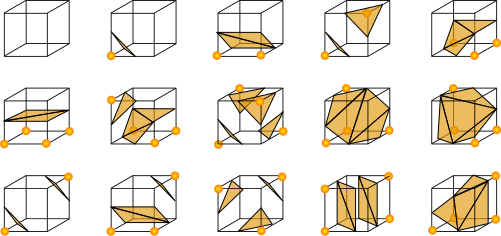
\includegraphics[scale=0.7]{figures/MarchingCubes}\caption{Triangulation for the 15 patterns. \label{fig:Marching cubes}}
\end{figure}
\indentTo visualization the model, obtained by marching cubes, the
VTK library is used, which enables building the three-dimension model.
\\
\indent The second part of this module includes visualization of the
brain's cross-section on arbitrarily defined plane. \\
\indent

There are three primary imaging planes that are performed in medical
imaging:
\begin{itemize}
\item axial plane, which is any plane that divides the body into superior
and inferior parts, roughly perpendicular to spine.
\item sagittal plane, which is any imaginary plane parallel to median plane.
\item coronal plane, which is any vertical plane that divides the body into
anterior and posterior sections.
\end{itemize}
The MRI produces two-dimensional images that consist of slices of
brain's and is usually performed in axial plane. To receive images
in the remaining planes, linear interpolation is used 

\section{Module 11}

-detailed description of module, algorithm etc, NO CODES, only theoretical!

\chapter{Implementation}

\section{Tools}

-python version, libraries

\section{Module 1}

-code

\section{Module 2}

-code
\section{Module 3}

-code
\section{Module 4}

-code
\section{Module 5}

-code
\section{Module 6}

-code
\section{Module 8}

-code
\section{Module 9}

-code
\section{Module 10}

-code
\section{Module 11}

-code

\chapter{Tests}

\section{Module 1}
-module 1 tests
\section{Module 2}
\section{Module 3}
\section{Module 4}
\section{Module 5}
\section{Module 6}
\section{Module 8}
\section{Module 9}
\section{Module 10}
\section{Module 11}
\section{Application}
-whole app tests

\chapter{Authors}
Authors of this project are students of Biomedical Engineering, AGH UST, Krakow, Poland. 
\\
\begin{center}
\begin{tabular}{|c|c|}
\hline 
Name & Role \tabularnewline
\hline 
\hline 
Sylwia Mól & Project Manager\tabularnewline
\hline 
 Jacek Fidos &  Software architect\tabularnewline
\hline 
Maciej Gryczan &  GUI engineer\tabularnewline
\hline 
Adrian Stopiak &  Vizualization engineer \tabularnewline
\hline 
Malwina Molendowska &  1st module developer \tabularnewline
\hline 
Klaudia Gugulska &  2nd module developer \tabularnewline
\hline 
Kacper Turek &  3rd module developer \tabularnewline
\hline 
Magdalena Rychlik &  4th module developer \tabularnewline
\hline 
Alicja Martinek &  5th module developer \tabularnewline
\hline 
Mateusz Pabian &  6th module developer \tabularnewline
\hline 
Anna Grzywa &  8th module developer \tabularnewline
\hline 
Magdalena Kucharska &  9th module developer \tabularnewline
\hline 
Eliza Kowalczyk &  9th module developer \tabularnewline
\hline 
Karolina Gajewska &  10th module developer \tabularnewline
\hline 
Michał Kotarba &  11th module developer \tabularnewline
\hline 
\end{tabular}
\end{center}
\newpage{}

\listoffigures

\begin{comment}
\bibliographystyle{plain}
\bibliography{bibliografia}
\end{comment}

\end{document}
